

\newcommand{\degrees}{${}^\text{o}$}

\graphicspath{{figures/}}

\setcounter{chapter}{3}
\chapter{Modelling river temperature} 


%\begin{chapquote}{H\r{a}rvard Rue and Leonard Held, \textit{GMRFs: Theory and Applications}}
%A GMRF is a really simple construct: It is just a random vector following a multivariate normal distribution.
%\end{chapquote}


% ------------------------------------------------------
% ------------------------------------------------------

\section{Introduction}

\begin{itemize}
  \item Stream temperature plays an important role in the ecological health of streams and rivers.
  
  \item For salmon, increased stream temperature in summer has the greatest impact ... \cmnote{find refs}, but something like:  increased stress, decreased growth and in the extreme increased mortality.   Low temperatures also have implications, though less severe, but include ...

  \item One important regulator of stream temperature is shade provided by trees.  

  \item In the US, there has been a lot of work looking at the effects of clear felling on stream temperatures; because the removal of shading could result in higher stream temperatures \rfnote{refs see iain}.  In the UK attention has focused on the effects of planting near the banks of rivers on stream temperature as a mitigation for increasing temperatures due to climate change\rfnote{more refs - see iain, what has been found?}.
\end{itemize}

% ------------------------------------------------------
% ------------------------------------------------------




\subsection{Previous approaches}

\begin{itemize}
\item Previous studies see AGU presentation for examples of previous studies. Previous modelling approaches and experimental designs.
\end{itemize}

One approach based on a paired catchment design developed by Moore et al. (2005), developing previous work by Watson (2001), estimates the relationship between stream temperature at a control site and a study site using linear regression with auto-regressive residuals.  The relationship is fitted under natural conditions before any felling has taken place.  This baseline relationship is then used to predict the stream temperature at the study site after felling.  Any difference in the predicted (baseline) temperature and the recorded temperature is then interpreted as a result of the felling. 

The prefelling model takes the form
\begin{equation}
  y_i = a + b x_i + c_1 \sin\left( \frac{2 \pi \text{doy}_i}{365} \right) + 
                    c_2 \cos\left( \frac{2 \pi \text{doy}_i}{365} \right) + ar_k(\text{day}_i)
\end{equation}
where $y_i$ is the $i$th observation of daily mean stream temperature at the impact site and $x_i$ the same for the control site, for $i = 1, \ldots, n$.  The year and day of the year associated with the observations are doy${}_i$ and year${}_i$, additionally the number of days since the start of the study is required which is denotes day${}_i$. The $k$th order auto-regressive process $ar_k(j)$ can be defined as
\begin{equation}
  ar_k(j) = u_j = \phi_1 u_{j-1} + \ldots + \phi_k u_{j-k} + \epsilon_j
\end{equation}
where $j = 1, \ldots$ corresponds to consecutive days, and the error term $\epsilon_j$ is assumed to be iid normal
\begin{equation}
  \epsilon_j \sim \NormD(0,\, \sigma)
\end{equation}
That is the residuals are modelled as an AR($k$) process, and the seasonal trend as a sinusoid.  A felling effect is then implied by using this model to predict daily mean temperatures after the impact and inspecting the residuals
\begin{equation}
  y_i^* - \hat{y_i^*}
\end{equation}

There is no formal assessment of the significance of a felling effect, although it is inferred if the residuals are greater than that expected by prediction intervals for the stationary distribution of the fitted AR(k) process. In the applications in Moore et al. (2005) the prediction intervals were approx +/- X\cmnote{get from Moore paper} degree.

The attractiveness of this approach is that it does not make any parametric assumptions about the effect of felling.

However, a limitation of existing methods is that they do not allow for a quantitative assessment of the magnitude of the felling effect or for the speed of recovery as trees are replanted 

For computational reasons, most current model based assessments of felling use daily summary data such as the daily mean, minimum or maximum temperature.  Often, up to 96 daily observations are reduced to one or two summary measures, which are then modelled and interpreted in turn.  This gives limited insight into the effect of felling on the cyclical within-day (or diel) changes in temperature.  For example, they would not be able to estimate the length of time that a stream is above a critical temperature, say, but are restricted to statements about daily maximums or daily means.

% ------------------------------------------------------
% ------------------------------------------------------



\subsection{Chapter structure}

This chapter develops new methods for quantifying the effect of clear felling on stream temperature and the speed of recovery.  It assumes that there are temperature time series from two streams (a paired catchment study), a control stream with no felling activity, and an impacted stream with data from both before and after a clear felling event.  The methods can be used with daily temperature summaries, but can also be used to estimate the effects of felling on diel variability in temperature.  The methods are illustrated using data from two burns in Loch Ard.

\textbf{Section 4.2} describes the data from Loch Ard.  

\textbf{Section 4.3} uses a subset of the data to formulate a simple model that motivates the subsequent methodological development.

\textbf{Section 4.4} develops models that formally assess the effect of felling. These models use cyclic smoothers (see chapter 2) to characterise seasonal variation. Felling is included as parametric function.  To account for short term climatological effects, an AR1 process (see chapter 2) is used.  I illustrate these fits using daily mean temperatures.

\textbf{Section 4.5} develops methods to model diel variation in temperature by extending the daily model from 4.4 through the use of functional data techniques.

\paragraph{Section 4.6} shows how these models can be used to predict the effect of felling for different temperature regimes, and hence show the range of effects from cold to warm days.  This is important for assessing the maximum impacts on stream temperature, and hence the risks for salmon under different scenarios.

% -------------------------------------------------------------------------
% -------------------------------------------------------------------------
% -------------------------------------------------------------------------
% -------------------------------------------------------------------------



\section{Data}

\subsection{Study site}

Stream temperature was monitored in two burns (Burns 2 and 10) in the Loch Ard area of West Central Scotland.  Figure \ref{fig:chptr4:sitemaps} shows the location of the site and where the stream temperature was monitored on Burn 10 (yellow dot). Burn 10 is a forested site within an area of managed woodland while burn 2 is an upland moor site.

% -------------------------------------------------------------------------
% -------------------------------------------------------------------------



\subsection{Felling event}

Figure \ref{fig:chptr4:fellingExtent} shows a map depicting a planned felling event that took place in Burn 10 in 2004.  The felling occurred to the south of the river and left a buffer zone of trees between the river and the clear felling area.  It is not known exactly when the felling took place, but evidence such as time series of nutrients in the water corroborate the year of the event.

% ------------------------------------------------------
\begin{figure}
\centering
  \begin{subfigure}[b]{0.4\textwidth}
    \centering
    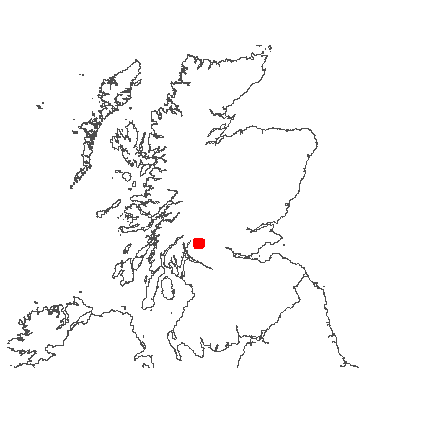
\includegraphics[width=\textwidth]{SiteMap}
    \caption{}
    \label{fig:chptr4:sitemap}
  \end{subfigure}
  \hfill
  \begin{subfigure}[b]{0.4\textwidth}
    \centering
    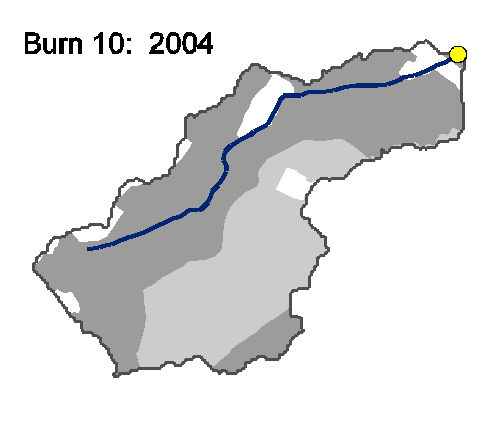
\includegraphics[width=\textwidth]{Burn10Felling2004}
    \caption{}
    \label{fig:chptr4:fellingExtent}
  \end{subfigure}
\caption{Study site and felling extent}
\label{fig:chptr4:sitemaps}
\end{figure}
% ------------------------------------------------------


% -------------------------------------------------------------------------
% -------------------------------------------------------------------------



\subsection{Temperature monitoring}

Stream temperature was monitored in the two catchments from 1999 to 2013.  The full time series of data is shown in Figure \ref{fig:chptr4:timeseries}. 

% ------------------------------------------------------
\begin{figure}
  \centering
  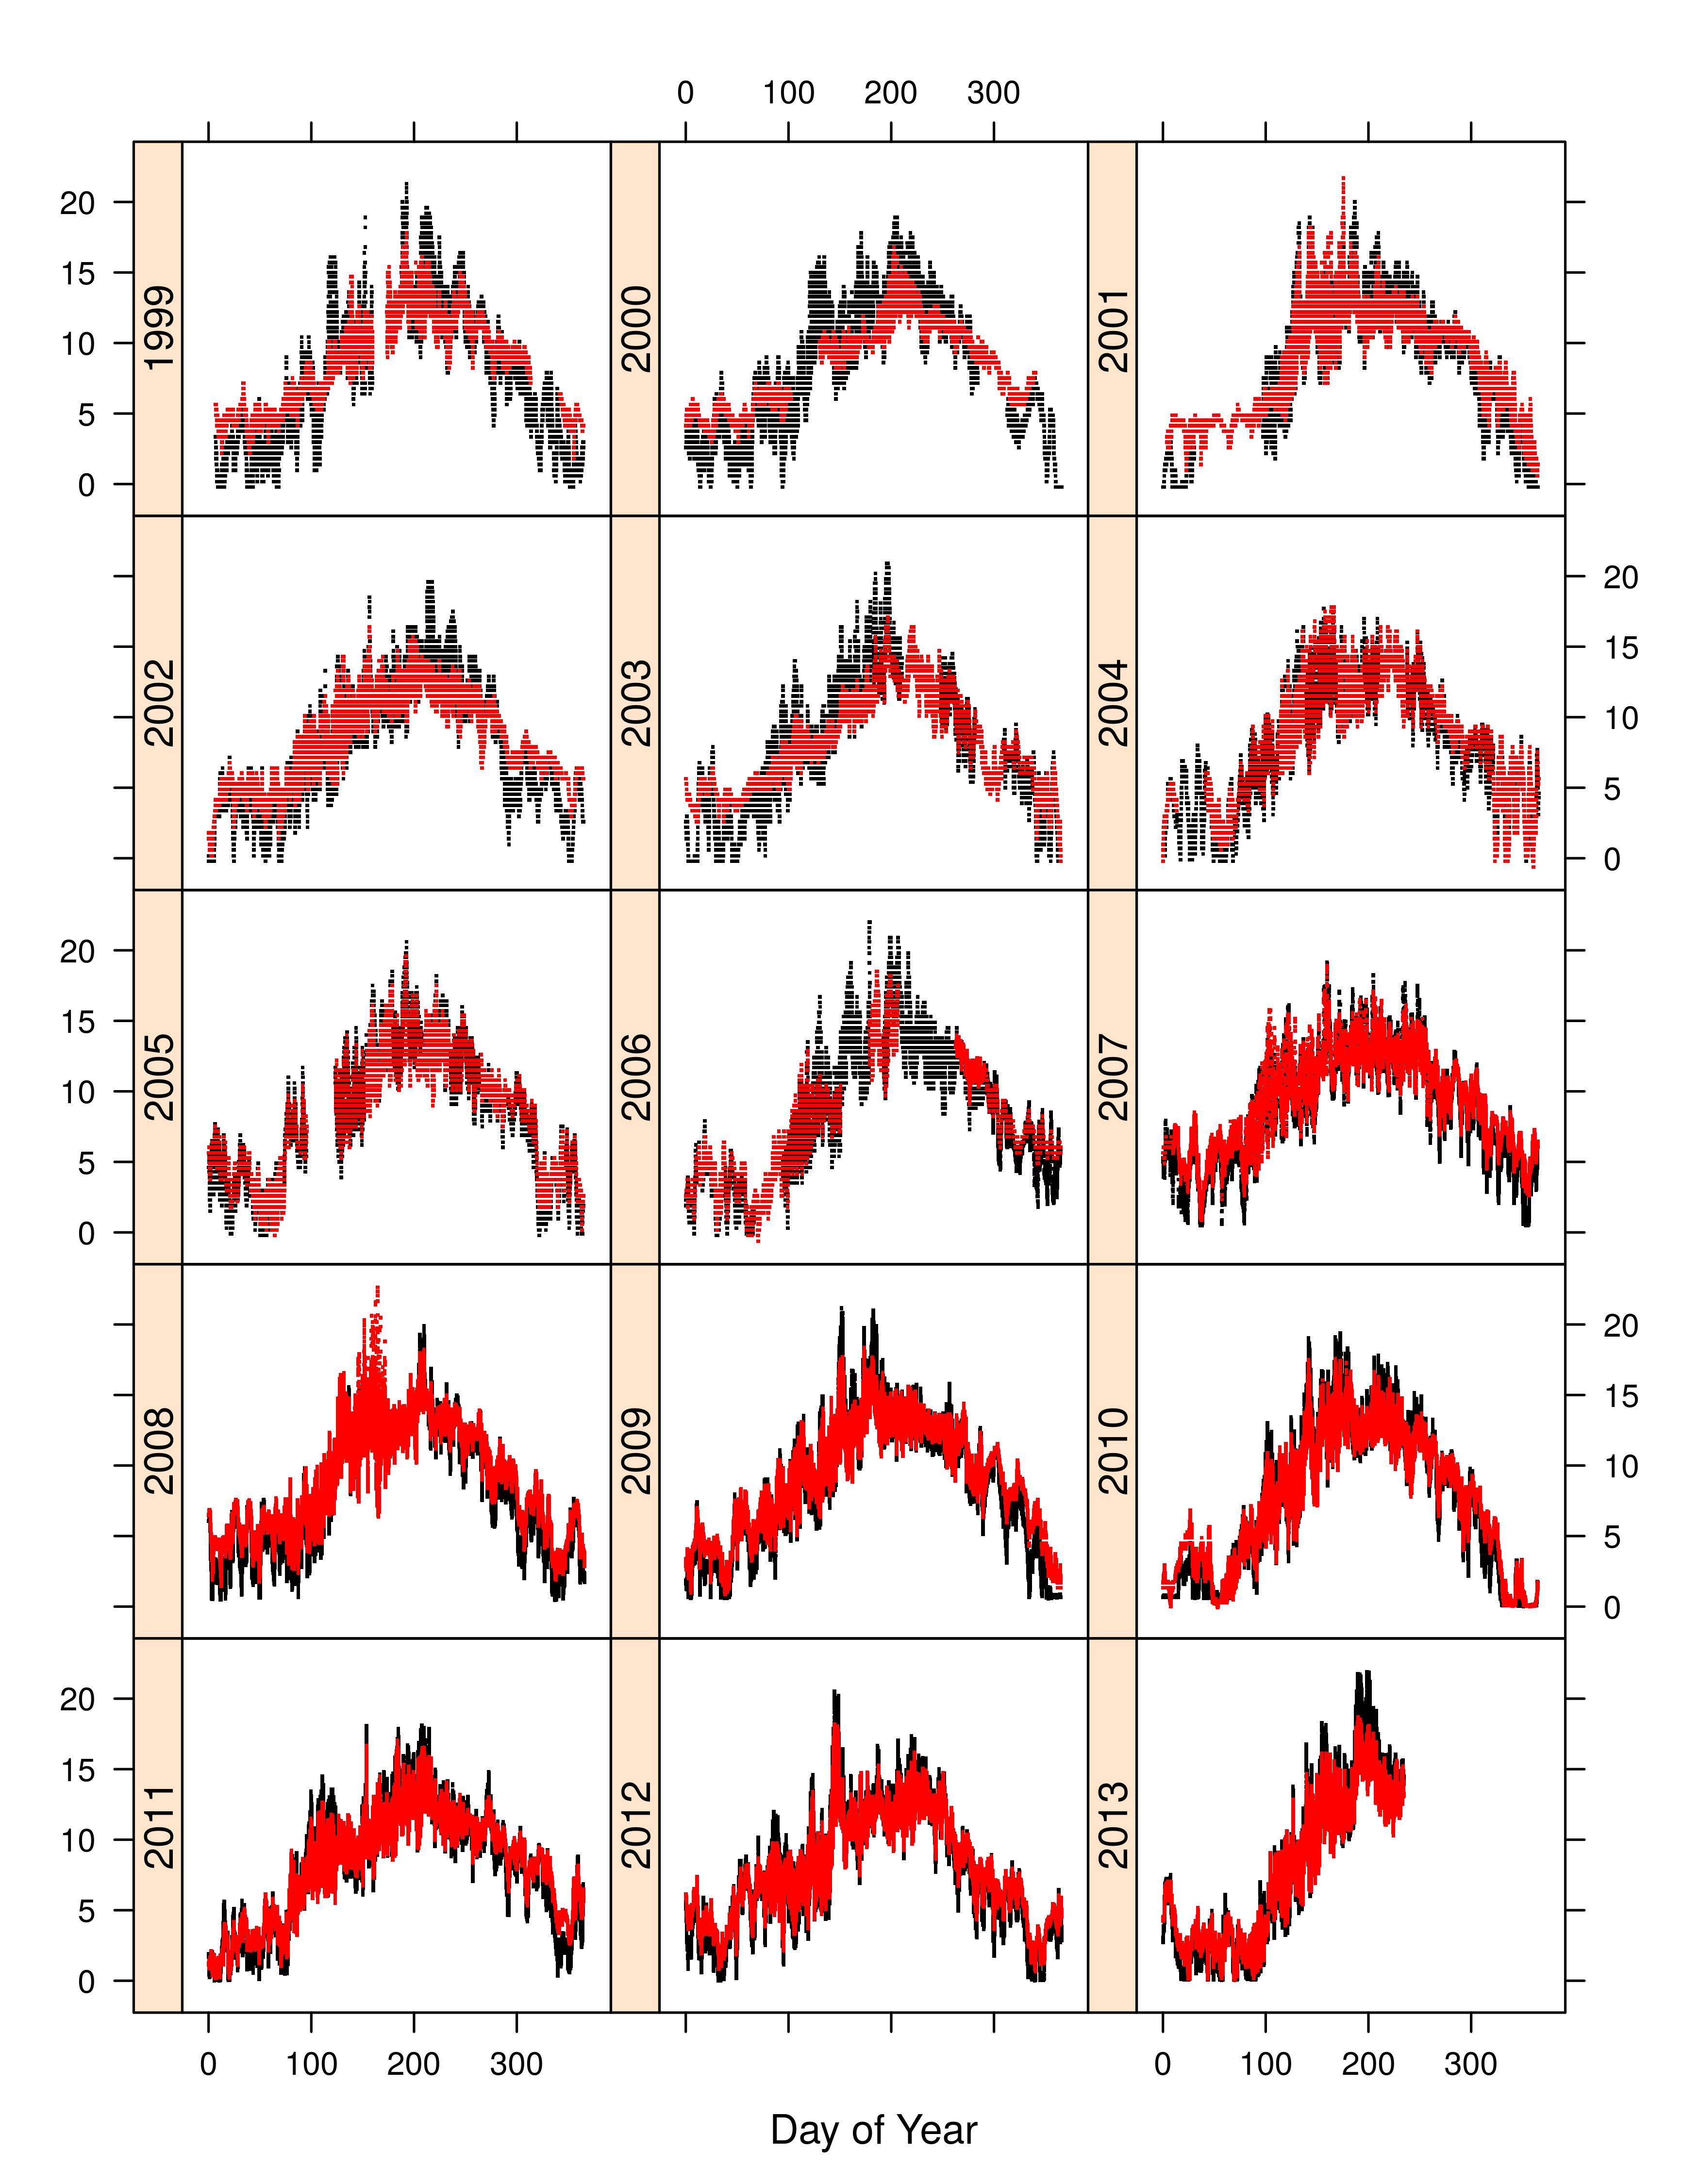
\includegraphics[height=0.9\textheight]{dataplot}
\caption{Time-series of temperature observations from Burns 2 and 10.}
\label{fig:chptr4:timeseries}
\end{figure}
% ------------------------------------------------------


A range of temperature dataloggers with various reporting resolutions (typically 0.01 - 0.2 \degrees C) were deployed over the study period. This can be seen in Figure \ref{fig:chptr4:timeseries}: data prior to 2008 shows as discretised (i.e. observations are rounded to increase the storage capacity of the loggers). Reporting frequency also varied from hourly to every 15 minutes. However, the same make and model of datalogger was deployed consistently over the two sites.

% -------------------------------------------------------------------------
% -------------------------------------------------------------------------



\subsection{Data cleaning}

Prior to analysis the data was screened to ensure as far as possible that the data is a true representation of the temperature in the stream.  Examples where data was removed was in winter when the stream froze and the thermistor (the temperature sensor) was exposed to the air or insulated by snow; during dry spells in the summer when the water level dropped below the level of the thermistor; and periods where the data-logger was clearly mis-calibrated (all temperatures were too high) in which case the time series of that particular logger deployment was removed. 

After cleaning the total number of paired observations was \cmnote{give an idea of the size of the dataset}

% -------------------------------------------------------------------------
% -------------------------------------------------------------------------



\section{Simple motivating model}
\label{sec:chpt4:simple}

To motivate the problem, and to introduce notation, consider two streams within the same river catchment with characteristics similar to those in Scotland. Because they share a similar location and hence climate you might expect them to be similar in terms of stream temperature. However, due to differences such as the terrain of their catchments, altitude, orientation and forestation, there temperatures could be quite different.  They will, however, behave similarly as the major factor controlling stream temperature is radiation from the sun. It should then be possible to model the behaviour of one stream in terms of another, and this is the basis of paired catchment analyses such as Moore at al. (2005). 

To get a feeling for the relationship between streams I will begin by looking at the temperatures of our two study streams, Burn 2 and Burn 10, but restrict our investigation to a short period of time so we can ignore seasonal and temporal effects.  Figure \ref{fig:chptr4:simpleplot1a} plots the temperature in Burn 2 against Burn 10, according to measurements made during May 2003 (the year prior to the felling event).

% -------------------------------------------------------------------------
\begin{figure}
\centering
  \begin{subfigure}[b]{0.45\textwidth}
    \centering
    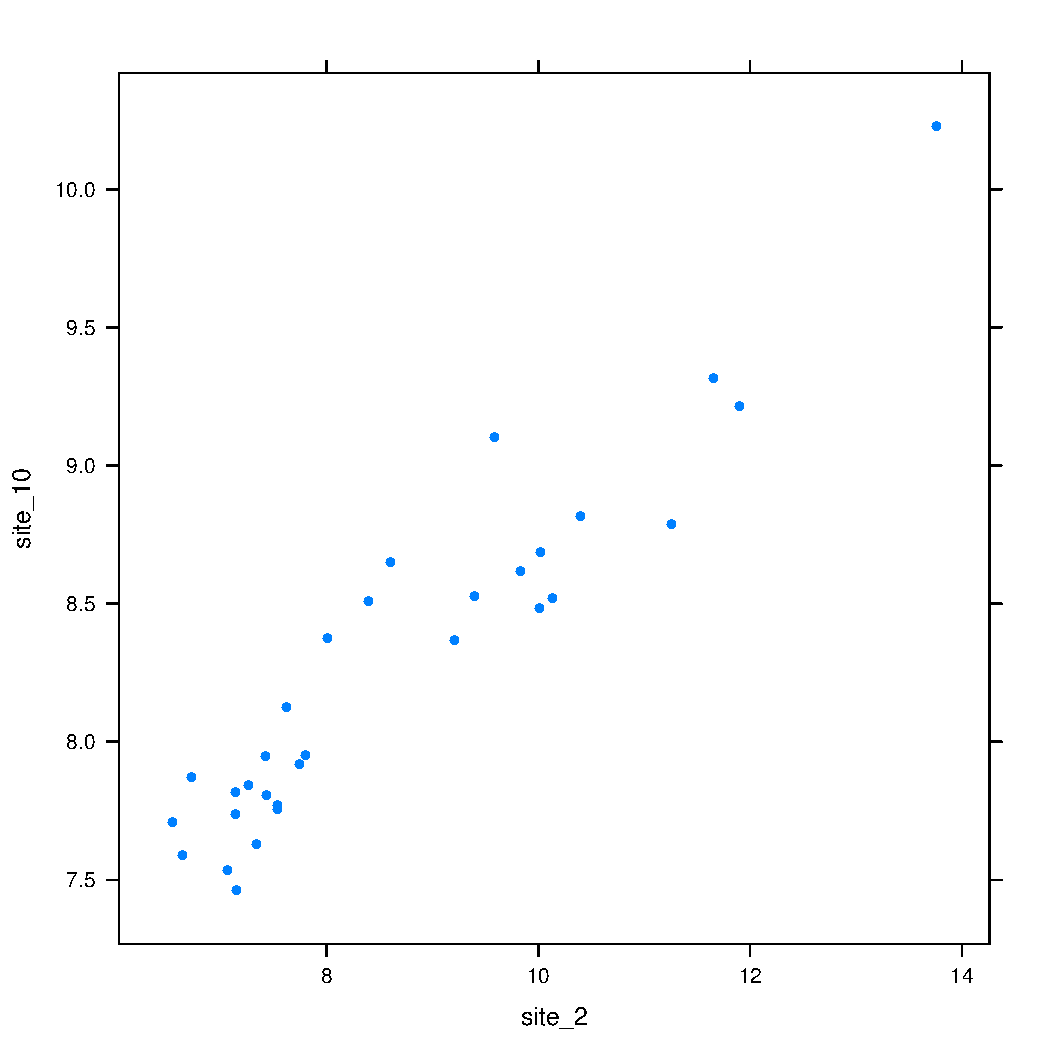
\includegraphics[width=\textwidth]{simpleExampleplot-1}
    \caption{Data from May 2003}
    \label{fig:chptr4:simpleplot1a}
  \end{subfigure}
  \hfill
  \begin{subfigure}[b]{0.45\textwidth}
    \centering
    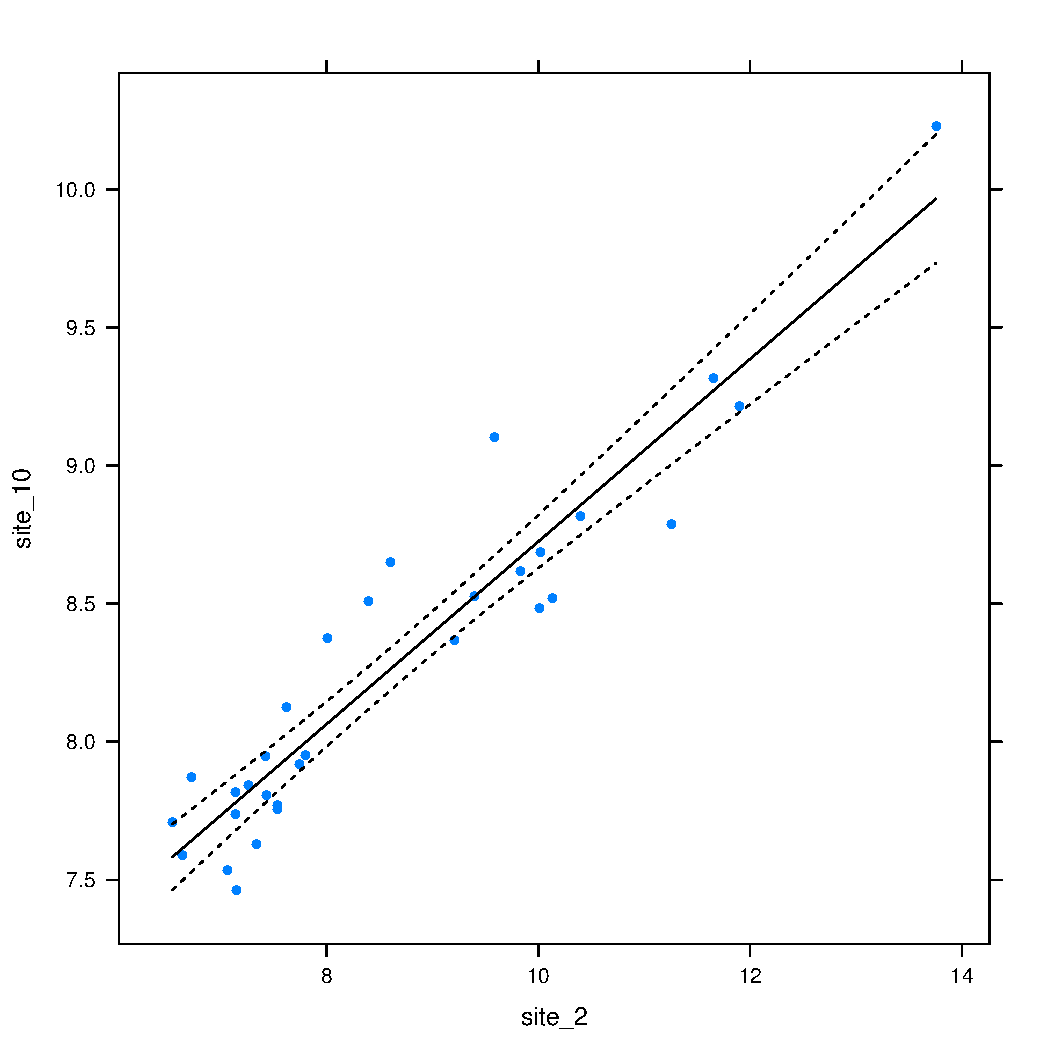
\includegraphics[width=\textwidth]{simpleExampleplot-2}
    \caption{data from May 2003 with a linear model fitted}
    \label{fig:chptr4:simpleplot1b}
  \end{subfigure}
\caption{Temperature observations from Burns 2 and 10 in May 2003.}
\label{fig:chptr4:simpleplot1}
\end{figure}
% -------------------------------------------------------------------------

% latex table generated in R 3.2.0 by xtable 1.7-4 package
% Sat May  9 09:23:49 2015
\begin{table}[ht]
\centering
\begin{tabular}{rrrrr}
  \hline
 & Estimate & Std. Error & t value & Pr($>$$|$t$|$) \\ 
  \hline
(Intercept) & 5.4210 & 0.1905 & 28.45 & 0.0000 \\ 
  site\_2 & 0.3304 & 0.0216 & 15.32 & 0.0000 \\ 
   \hline
\end{tabular}
\end{table}

The temperatures are clearly correlated, but burn 2 differs from burn 10 on average by 0.37 \degrees C\rfnote{Need to update these values} and occupies a different temperature range: 6.58 to 13.76 \degrees C, compared to 7.46 to 10.17 \degrees C for burn 10. It looks, from Figure \ref{fig:chptr4:simpleplot1a}, that a linear model could be a good way to characterise the relationship between the temperatures in the two streams. One way to proceed is to consider the linear model 
\begin{equation}
  y_i = a + b x_i + \epsilon_i
\end{equation}
where $i = 1, \ldots, 31$ denotes the days of the month under study
\begin{equation}
  \epsilon_i \sim \NormD(0,\, \sigma)
\end{equation}

Prior to analysis all temperatures have been centred around the mean daily temperature which for the time series is 7 \degrees C.  Hence, $y_i$ is the $i$th  (paired) observation of centred daily mean temperatures in Burn 10, and $x_i$ is the same for Burn 2. We will ignore the fact $x_i$ is also observed with error, and assume for now that the residuals are iid normal with variance sigma.  This model can be written in matrix notation as follows:
\begin{equation}
  \bm{y} = \bm{X\beta} + \bm{\epsilon}
\end{equation}
where $\bm{y} = (y_1, y_2, \ldots, y_n)$, and $X$ is a two column matrix formed from a column of 1s for the intercept $a$ and $\bm{x} = (x_1, x_2, \ldots, x_n)$. The parameters in the linear model are easily estimated using maximum likelihood estimator
\begin{equation}
  \hat{\bm{\beta}} = \Big(\bm{X}'\bm{X}\Big)^{-1} \bm{X}' \bm{y}
\end{equation}
to be $a$ = 5.45 and $b$ = 0.33. This means that for every 1 \degrees C change from a the average 7 \degrees C daily mean in Burn 2, Burn 10 changes by 0.33 \degrees C.  This is interesting as the catchment\rfnote{earlier you said they are the same catchment} for Burn 2 is moorland, whereas the catchment for Burn 10 is forested; the lack of river shading in Burn 2 seems to result in higher stream temperatures.

% -------------------------------------------------------------------------
\begin{figure}
\centering
  \begin{subfigure}[b]{0.45\textwidth}
    \centering
    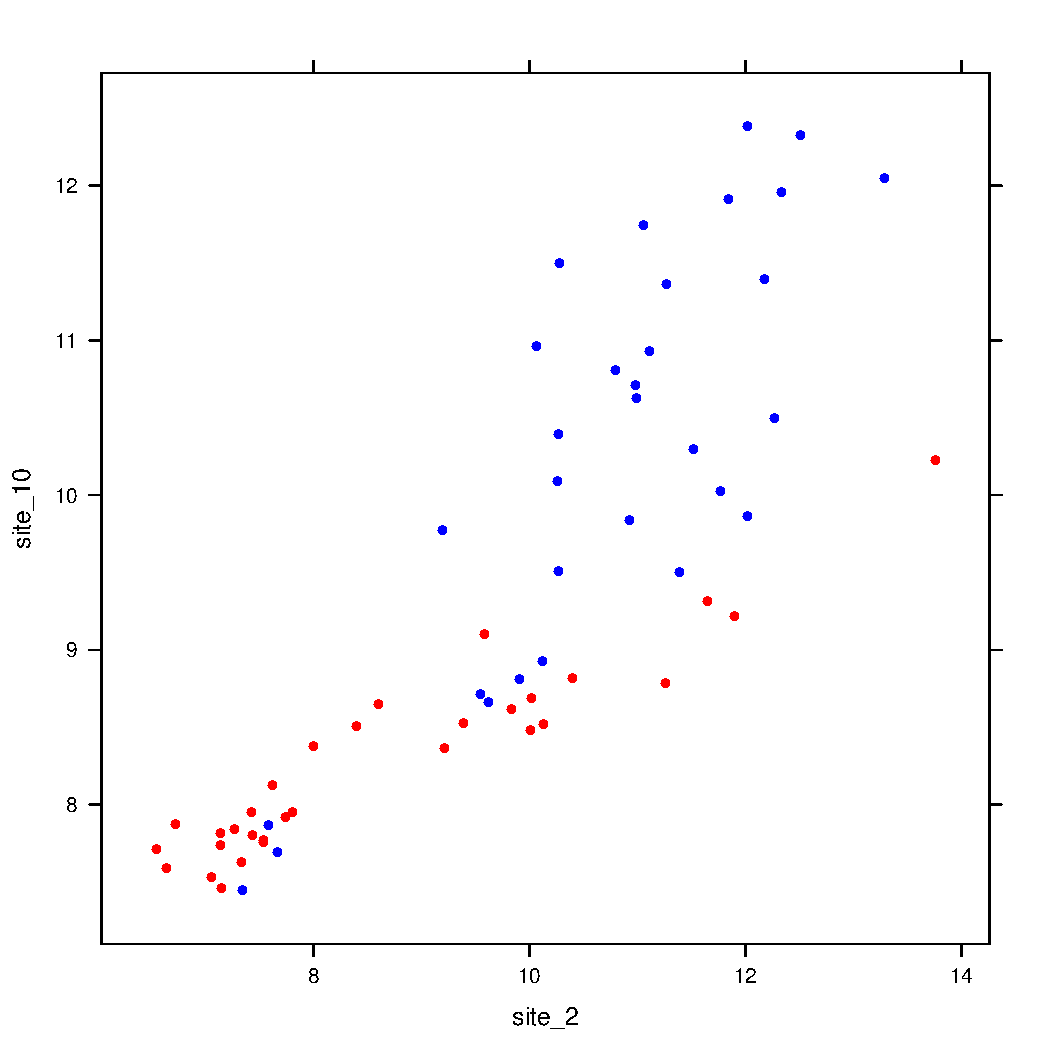
\includegraphics[width=\textwidth]{simpleExample2plot-1}
    \caption{Data from May 2003 and 2004}
    \label{fig:chptr4:simpleplot2a}
  \end{subfigure}
  \hfill
  \begin{subfigure}[b]{0.45\textwidth}
    \centering
    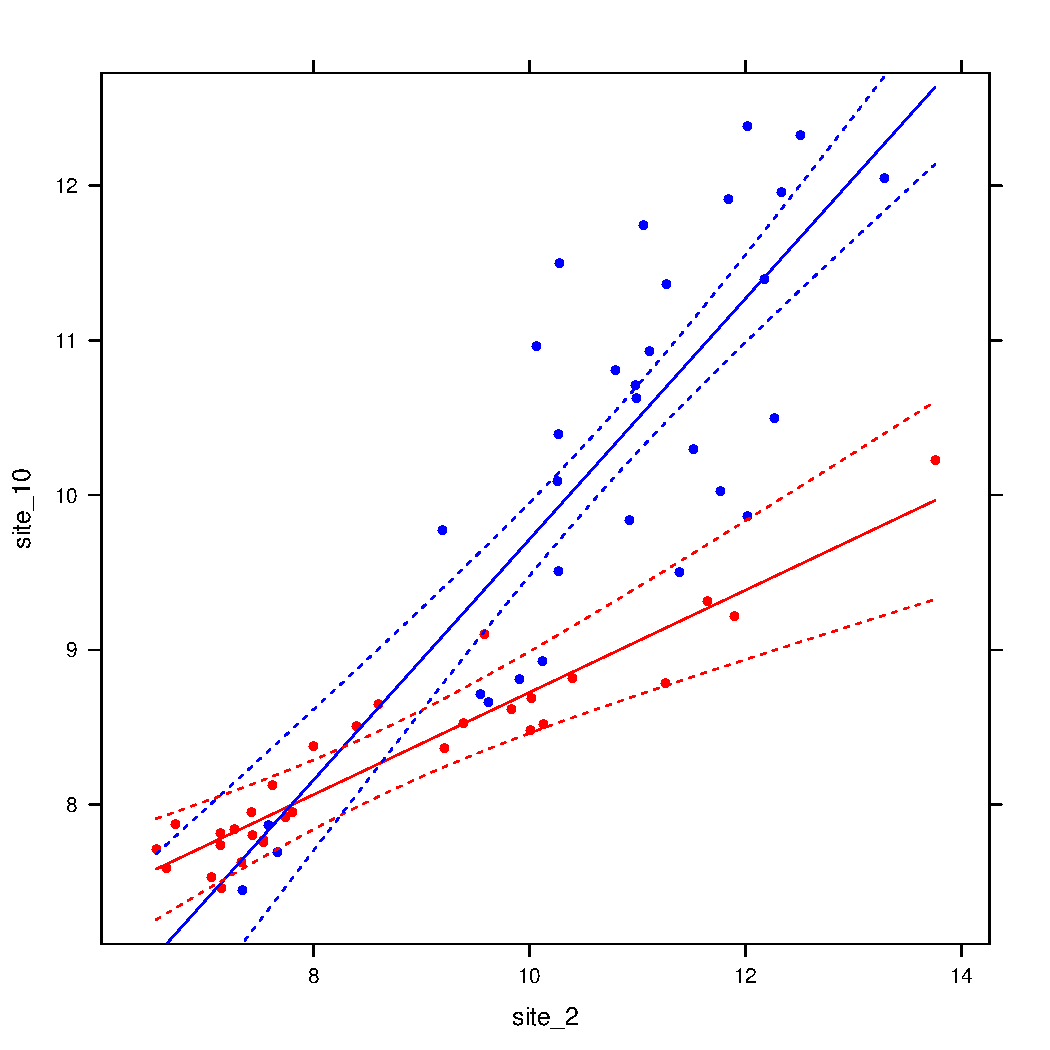
\includegraphics[width=\textwidth]{simpleExample2plot-2}
    \caption{data from May 2003 with a linear model fitted}
    \label{fig:chptr4:simpleplot2b}
  \end{subfigure}
\caption{Temperature observations from Burns 2 and 10 in May 2003 and May 2004.}
\label{fig:chptr4:simpleplot2}
\end{figure}
% -------------------------------------------------------------------------

% latex table generated in R 3.2.0 by xtable 1.7-4 package
% Sat May  9 09:26:32 2015
\begin{table}[ht]
\centering
\begin{tabular}{rrrrr}
  \hline
 & Estimate & Std. Error & t value & Pr($>$$|$t$|$) \\ 
  \hline
(Intercept) & 5.4210 & 0.5223 & 10.38 & 0.0000 \\ 
  site\_2 & 0.3304 & 0.0591 & 5.59 & 0.0000 \\ 
  felling & -3.4869 & 0.9584 & -3.64 & 0.0006 \\ 
  site\_2:felling & 0.4476 & 0.0949 & 4.71 & 0.0000 \\ 
   \hline
\end{tabular}
\end{table}


The felling event which is the focus of this chapter took place in the subsequent year (2004) in the catchment of Burn 10 (Figure \ref{fig:chptr4:fellingExtent}). The data plotted in Figure \ref{fig:chptr4:simpleplot2} indicates that there was an effect of the clear felling on the daily mean temperatures. One way to quantify the effect of this felling on stream temperature in burn 10 is to introduce a parameter for felling: 
\begin{equation}
 \label{eq:chtr4:simplemod2}
 y_{ij} =
  \begin{cases}
   a + b x_{ij} + \epsilon_{ij}                    & \text{if } j = 2003 \\
   a + b x_{ij} + \underbrace{a_f + b_f x_{ij}}_\text{felling effect} + \epsilon_{ij} & \text{if } j = 2004 
  \end{cases}
\end{equation}
where $i=1, \ldots, 31$\cmnote{Need to change this notation slightly} denotes the days of the month under study, and $j = 2003, 2004$ are the years considered.  The residual variance is assumed to be constant.
\begin{equation}
  \epsilon_{ij} \sim \NormD(0,\, \sigma)
\end{equation}
Figure \ref{fig:chptr4:simpleplot2} shows stream temperatures from 2003 and 2004 with the fitted line from (\ref{eq:chtr4:simplemod2}). The model can again be written in the matrix form as before, hence the same maximum likelihood estimator of the parameters applies, the difference being that this model has a design matrix $\bm{X}$ with 4 columns. The estimates of the felling parameters are $a_f$ = -1.55 (-2.65, -0.49) and $b_f$ = 0.26 (0.13, 0.37); the values in brackets are the 95\% confidence intervals derived from the estimate of the variance of b which is given by the 4 x 4 matrix
\begin{equation}
  \bm{V} = \Big(\bm{X}'\bm{X}\Big)^{-1}
\end{equation}
The effect of felling on the intercept and slope in this model has a high probability of being non-zero and hence we conclude that there is a significant felling effect. Note that the slope has changed from 0.33 to 0.58 - so the  removal of trees has made the temperatures in burn 10 more similar to that in burn 2 (because it is closer to 1).  We can also predict, with confidence intervals, the effect of felling experienced during May of 2004 from the following
\begin{equation}
  \text{felling} = a_f + b_f \bm{x} = \bm{X}_f \bm{\beta}
\end{equation}
Confidence intervals can be derived for the felling effect by linear transformation of the variance
\begin{equation}
  \bm{X}_f \bm{V} \bm{X}'_f
\end{equation}
where $\bm{X}_f$ is the design matrix from the model with the first two columns set to zero.  
The reason for the change in temperature is due to the removal of shading, increasing the amount of radiation received from the sun and hence increasing the stream temperature ($a_f$) and increasing the effect of increased sunshine ($b_f$).\cmnote{Perhaps a  small diagram from one of Iains papers to highlight what is going on.}

Shade reducing input from the sun is one aspect of the effect of forestation on stream temperature.  The other is that shade (through tree cover) also reduces heat loss and so on cold days the removal of trees would be expected to result in greater decreases in temperature.  To investigate this effect the model is extended to cover all the months in the year.
\begin{equation}
  y = \beta_a + \beta_b x + \beta_a(\text{moy}) + \beta_b(\text{moy})x + \epsilon
\end{equation}\cmnote{need to think about these equations, and improve the plot}
The fits from the model are shown in Figure \ref{fig:chptr4:monthlyfits}, and shows there is apparent seasonality in the intercept and potentially in the slope.  The felling effect also appears to vary seasonally.

% -------------------------------------------------------------------------
\begin{figure}
  \centering
  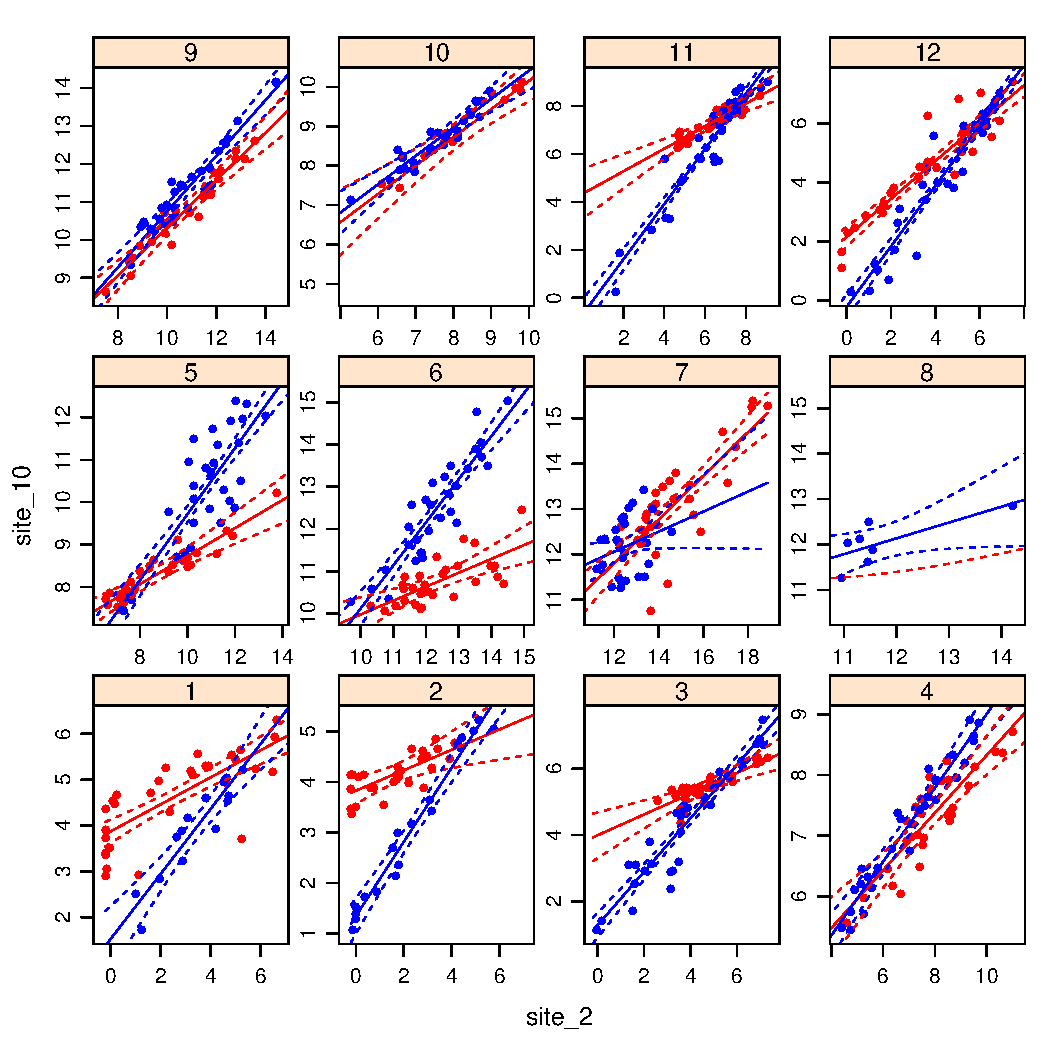
\includegraphics[width=\textwidth]{simpleExample3plot-2}
\caption{Monthly fits}
\label{fig:chptr4:monthlyfits}
\end{figure}
% -------------------------------------------------------------------------


This basic approach forms the basis that will be used to estimate the effect of felling in the more complex situation where the relationship between sites varies continuously and where the effect of felling is estimated for multiple years allowing for the possibility that the felling effect gradually reduces through time as vegetation and trees regrow returning levels of shading back to that prior to felling.


% -------------------------------------------------------------------------
% -------------------------------------------------------------------------
% -------------------------------------------------------------------------
% -------------------------------------------------------------------------





\section{Modelling daily felling effects}

Preliminary analysis in Section \ref{sec:chpt4:simple} showed that a linear relationship holds between sites when viewed on a month by month basis (Figure \ref{fig:chptr4:monthlyfits}). The models developed in this section for a felling effect are the same in spirit as the simple example: define a baseline model and a model for a felling effect in which the pre-felling data is given by the baseline state which is then augmented by a felling effect to model the post felling data.

This section further extends this simple idea to allow for a felling effect which decays over time in several ways.  GCV is used as the fitting criterion at each stage and also serves to highlight were additions to the felling decay model provide improved fits.

% -------------------------------------------------------------------------
% -------------------------------------------------------------------------



\subsection{Simple model}


The structural form of a relationship between two streams is likely to be seasonal as shown in Figure \ref{fig:chptr4:monthlyfits}.  I use the following model which is a generalisation of that used by Moore at al.
\begin{equation}
  y = \beta_a + \beta_b x + g_a(\text{doy}) + g_b(\text{doy})x + \epsilon
\end{equation}
y is the mean daily temperature at Burn 10 centered by 7 \degrees C; 7 \degrees C is about the average stream temperature across the whole year. Similarly, x is the mean daily temperature at Burn 2 also centred by 7 \degrees C. The function $g_a(\text{doy})$ is the seasonal non-linear effect of doy (day of the year) for an average day.  The term $\beta_b + g_b(\text{doy})$ can be interpreted as the seasonal non-linear effect for every degree difference from an average day.  This model allows for a seasonal difference between Burn 2 and Burn 10 and a seasonal difference in how warmer or cooler temperatures in Burn 2 translate to Burn 10. The slope can also be thought of as how reactive to changes in temperature Burn 10 is, compared to Burn 2.

I use cyclic smoothers to model the functions $g_a$ and $g_b$ which are common across years. First let's consider a full rank GMRF smoother. Let the vector $\bm{\gamma}_a = (\gamma_{a,1}, \ldots, \gamma_{a,365})$ represent the daily seasonal effect of day of the year described by the function $g_a(\text{doy})$. Then, in matrix notation, the effect on any given day is given by $\bm{Z}_i \bm{\gamma}_a$, where $\bm{Z}_i$ is a (row) vector of length 365, with a 1 in the column for the appropriate day and zeros elswhere, so for the if the $i$th observation took place on the 40th day of the year, $Z_{i,40}$ is 1, and $Z_{i,j}$ for $j \neq 40$ is 0.  This allows a design matrix to be specified for the days on which paired observations took place, so that the function $g_a$ can be evaluated at an arbitrary subset of days of the year through   
\begin{equation}
  g_a(\text{doy}) = \bm{Z}_a \bm{\gamma}_a
\end{equation}

For the interaction term $g_b(\text{doy})\text{ cburn2}$, a similar approach can be taken.
Let the centered burn 2 daily mean temperatures be denoted by $x_{ij}$).  Then the interaction term effect on any given day $i$ in any year $j$ is $x_{ij} \bm{Z}_i \bm{\gamma}_b$, so that the burn 2 temperatures can be absorbed into the design matrix
\begin{equation}
  g_b(\text{doy})\text{ cburn2} = \bm{Z}_b \bm{\gamma}_b
\end{equation}
The intercept and slope terms $\beta_a$ and $\beta_b$ can also be writted in matrix notation. The vector equation for the centered daily mean temperatures in burn 10, $\bm{y}$ is
\begin{equation}
  \bm{y} = \bm{Z}_a \bm{\gamma}_a + \bm{Z}_b \bm{\gamma}_b + \bm{X} \bm{\beta} + \bm{\epsilon}
\end{equation}

% -------------------------------------------------------------------------



\subsubsection{Smoother choice}

The seasonal effect can be achieved through the use of a variety of penalties. Possible approaches include the 1st order cyclic random walk GMRF models (CRW1) as described in chapter 2.  While  another is to use a harmonic oscillator penalty (HO). The CRW1 model is based on penalising day to day changes in temperature where there is an explicit link between the last day in the year and the first day in the year.  In terms of derivatives, this model is based on penalising 1st differences, and can be written in terms of a differential operator $\bm{D}$

\begin{equation}
  \bm{D}g = g'(\text{doy})
\end{equation}

In the discrete time case, the operator $\bm{D}$ is a matrix which computes the differences between each day, and because the 365th day is linked to the 1st day, the last row of $\bm{D}$ computed this difference. The discrete (cyclic) differential operatior is the $n \times n$ matrix
\begin{equation}
\bm{D} = 
\begin{pmatrix} 
-1 & 1 &  &  &  &  &  \\ 
 & -1 & 1 &  &  &  &  \\ 
 &  &  & \ddots & \ddots &  &  \\ 
 &  &  &  &  & -1 & 1 \\ 
1 &  &  &  &  &  & -1 \\ 
\end{pmatrix}
\end{equation}
This basic operator can be used to define several cyclic smoothers.  The cyclic 1sy order random walk is given by the quadratic penalty ($\bm{D}'\bm{D}=\bm{Q}_{crw1}$), which is invariant to the additon of a constant term to the functon $g$. 
\begin{equation}
\bm{Q}_{crw1} = 
\begin{pmatrix} 
2 & -1 &  &  &  &  & -1 \\ 
-1 & 2 & -1 &  &  &  &  \\ 
 & -1 & 2 & -1 &  &  &  \\ 
 &  & \ddots & \ddots & \ddots &  &  \\ 
 &  &  & -1 & 2 & -1 &  \\ 
 &  &  &  & -1 & 2 & -1 \\ 
-1 &  &  &  &  & -1 & 2 \\ 
\end{pmatrix}
\end{equation}

The harmonic oscilator on the otherhand, penalises the 1st and 3rd derivatives together forming a penalty that is invariant to the addition of a phase shifted sine wave $a \sin(\omega x + \phi)$.  The appropriate penalty is based on the famous wave equation and is defined through a combination of differences using a linear differential operator $L$
\begin{equation}
  \bm{L}g = \bm{D}^{3}g + \omega^2\bm{D}g
\end{equation}
where $\omega$ is the period. The quadratic penalty for this is simply ($\bm{L}'\bm{L}=\bm{Q}_{harm}$).

\begin{equation}
\bm{Q}_{harm} = 
\begin{pmatrix} 
20 & -15 & 6 & -1 &  &  &  & -1 & 6 & -15 \\ 
-15 & 20 & -15 & 6 & -1 &  &  &  & -1 & 6 \\ 
6 & -15 & 20 & -15 & 6 & -1 &  &  &  & -1 \\ 
-1 & 6 & -15 & 20 & -15 & 6 & -1 &  &  &  \\ 
 & \ddots & \ddots & \ddots & \ddots & \ddots & \ddots & \ddots &  &  \\ 
 &  & -1 & 6 & -15 & 20 & -15 & 6 & -1 &  \\ 
 &  &  & -1 & 6 & -15 & 20 & -15 & 6 & -1 \\ 
-1 &  &  &  & -1 & 6 & -15 & 20 & -15 & 6 \\ 
6 & -1 &  &  &  & -1 & 6 & -15 & 20 & -15 \\ 
-15 & 6 & -1 &  &  &  & -1 & 6 & -15 & 20 \\ 
\end{pmatrix}
\end{equation}


Both these models require a parameter vector $\bm{\gamma}_a$ with 365 elements - a parameter for each day - which would be penalised by a 365x365 matrix.  For this moderate sized problem, the dimension of the smoothing matrix makes for slow computation.  In order to speed up the fitting process a reduced rank smoother (chapter 2) can be used.  

Reduced rank smoothers provide a means to reduce the number of parameters in a model by reducing the maximum model space.  However, the process involves computing the eigen decomposition of the penalty matrix, which again comes with computational cost.  There is a short cut by noticing the form of the new bases induced by diagonalising the penalty matrix.  Recall from chapter 2, that the \textit{best} parameterisation of a smoother could be achieved by transforming the parameter space so that the smoothing matrix was diagonal.  Wood (2006) called this the \textit{natural parameterisation} for a smoother, and it is appealing becuase the new basis functions contribute independently to the complexity of the fit.  With a diagonal penalty matrix, the smoothing problem becomes almost a ridge regression.

Consider the GMRF smoother for a discrete time process composed of n time points. The basis functions for this model are coded by the identity matrix, each point in the process has a single basis vector, much like the basis vectors $(i, j, k)$ for points in euclidean 3 dimensional space. Following the procedure for reduced rank smoothers, the penalty $g'Qg$ can be written $g'U'VUg$, by replacing $Q$ with its eigen decomposotion, so a transformed model with diagonal penalty matrix $V$ is
\begin{equation}
  y = Ug + e
\end{equation}
where $U$ defines the new basis functions.  The form of these basis functions is very insightful and are given in Figure \ref{fig:chptr4:eigenBasis} for the two GMRF smoothers (1st order cyclic random walk and the harmonic occilator random walk).

\begin{figure}
  \centering
  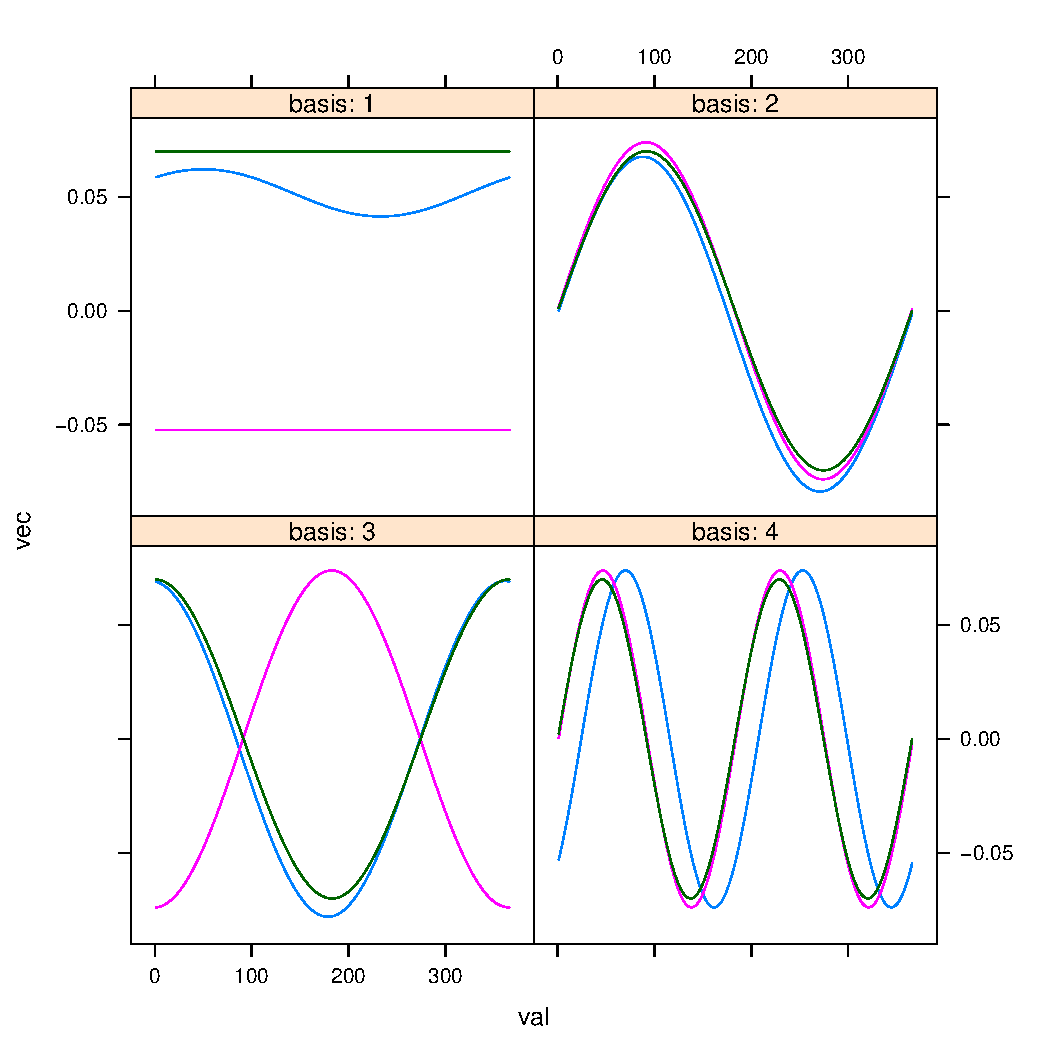
\includegraphics[width=\textwidth]{eigendecomp}
\caption{The first three basis functions of four GMRF models transformed to thier \textit{natural parameterisation}}
\label{fig:chptr4:eigenBasis}
\end{figure}

Notice that the basis function of the CRW1, harm are sine and cosine functions, hence the reduced rank models are intimately related to penalised splines based on fourier basis functions. In fact, the first 4 basis functions of the CRW1 penalty results in the first 4 discrete fourier basis functions. The harmonic basis functions are very similar to the CRW1 apart form of the 1st basis function which has a sinusoid form.

To investigate the utility of each approach the following model was fitted to the full time series of data
\begin{equation}
  y = a + x + g_a(doy) + \epsilon
\end{equation}
with 6 forms for the function $g_a$: 1) CRW1, 2) reduced rank CRW1 with 52 bases, 3) harmonic, 4) reduced rank harmonic with 52 bases, 5) one value for each week, and 6) cyclic cubic regression spline with 52 bases.  52 was chosen to restric the smoothness to to a weekly level. Figure \ref{fig:chptr4:smoothchoice} shows the fitted smoothers.  The results from CRW1, reduced CRw1, harm, and CC are very similar, the factor model is very wiggly as expected, while the reduced harm is also very wiggly.  The edf of the least wiggly models are range between 22 to 27 (Table \ref{tab:chptr4:efd}), with the harmonic models ataining the lowest smoothing parameter and among the lowest GCV.  Interesingly, the reduced harmonic model with 52 basis functions does not find the optimum smoother, but the reduced harmonic smoother with 100 basis functions does.  The lowest GCV actually came from the reduced rank CRW1 model.

% -------------------------------------------------------------------------
\begin{table}[ht]
\label{tab:chptr4:efd}
\centering
\begin{tabular}{l|l|l}
\hline
model & edf & gcv\\
\hline
crw1 & 27.258 & 0.54106\\
\hline
harm & 21.848 & 0.54009\\
\hline
factor & 52 & 0.54478\\
\hline
rrcrw1 & 25.589 & 0.54004\\
\hline
rrharm & 50.948 & 0.54308\\
\hline
rrharm100 & 21.854 & 0.54009\\
\hline
\end{tabular}
\end{table}
% -------------------------------------------------------------------------



% -------------------------------------------------------------------------
\begin{figure}
  \centering
  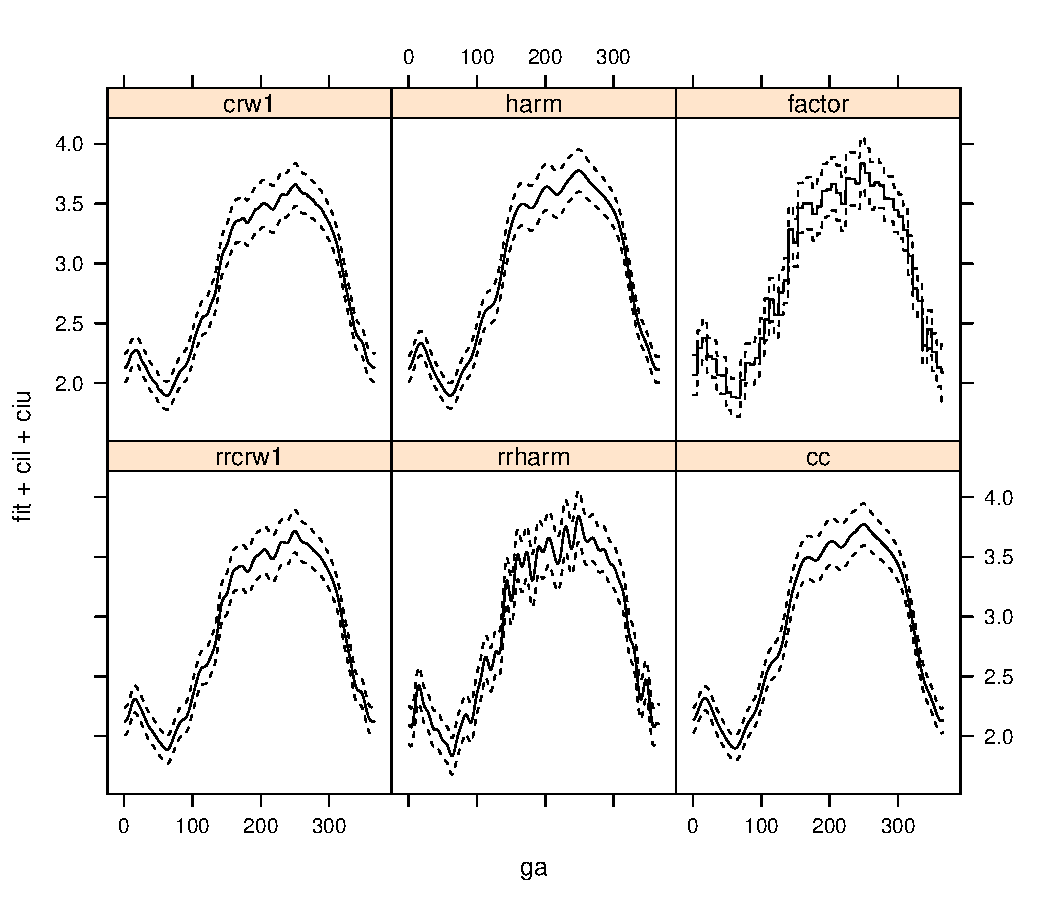
\includegraphics[width=\textwidth]{smoothChoice}
\caption{Monthly fits}
\label{fig:chptr4:smoothchoice}
\end{figure}
% -------------------------------------------------------------------------


% -------------------------------------------------------------------------



\subsubsection{Model fitting}

The coefficients $\bm{\gamma}_a$ and $\bm{\gamma}_b$ are then estimated using penalised least squares where the penalties are included as 
\begin{equation}
  \lambda_a \bm{\gamma}'_a \bm{Q}_{crw2} \bm{\gamma}_a + \lambda_b \bm{\gamma}'_b \bm{Q}_{crw2} \bm{\gamma}_b
\end{equation}

To estimate the parameters of the model for a given set of smoothing parameters, the maximum penalised log-likehood that is minimised is
\begin{equation}
  l^p(\bm{\gamma}_a, \bm{\gamma}_a, \bm{\beta}) = 
\end{equation}

For computational efficiency, rather then specify a full rank GMRF and reduce dimension, I simply use 52 fourier basis functions directly.  I choose 52 to allow for a maximum of weekly level variability, while still keeping the size of the model to a manageable size.  This choice of basis resonates well with the Moore et al. (2005) model which can be thought of as an unpenalised spline using the first 3 fourier basis functions. Because I am expressly seeking to model a sinusoidal function I use the harmonic penalty in conjunction with the fourier bases. \cmnote{Show a fit to the daily mean data.}

The model fits contain a lot of detail: they contain local (high frequency) time variations, where we are interested in longer range effects.  The use of multiple years of data should reduce problems with over-fitting, however, missing data in some years are perhaps causing over-fitting problems.

% -------------------------------------------------------------------------
% -------------------------------------------------------------------------




\subsection{adding AR1}

There are several ways to isolate long term trends.  This has been investigated by Cressie (find ref).  I implement a simple approach where local trends are assumed to be well described by a random stationary process, and hence possible models are auto-regressive process; in this application I use an AR1.  

It is possible to model the AR1 process in the model as an extra structural smoother. Because an AR1 process is a GMRF this precision matrix can be used directly as a penalty matrix.
\begin{equation}
\bm{Q}_{ar1}(\phi) = 
\begin{pmatrix} 
1 & -\phi &  &  &  \\ 
 -\phi& 1 + \phi & -\phi &  &  \\ 
 &  & \ddots &  &  \\ 
 &  & -\phi & 1 + \phi & -\phi \\ 
 &  &  & -\phi & 1 \\ 
\end{pmatrix}
\end{equation}
The model extended to include local variation is
\begin{equation}
  \text{cburn10} = \beta_a + \beta_b x + g_a(\text{doy}) + g_b(\text{doy})x + ar1(\text{doy}) + \epsilon
\end{equation}
The problem with this approach is that the size of the model increases with the number of observations so that fitting time becomes limiting.  The effect in this case is rather extreme as the AR1 process requires as many parameters as days.  The other problem is that the AR1 can be confounded with the observation error (i.e. the signal to noise ratio of the AR1 is not strong).  This can be remedied by fixing the regression error to a very small value, however, this can result in problems with parameter estimation if using GCV and would require switching to a criterion closely related to AIC called UBRE (UnBiased Risk Estimator).  However, in all these cases, the AR1 process is considered as part of the model and contributes to the model degrees of freedom.    

Since I am not interested in the AR1 inof itself, an alternative, used in many applications, is to model the residuals as AR1 directly.  In this model the AR1 process is imposed on the residuals by weighting the residuals in the fitting process using the square root of the precision matrix above, i.e. $\bm{Q}_{ar1} = \bm{D}_{ar1}'\bm{D}_{ar1}$ where,
\begin{equation}
\bm{D}_{ar1}(\phi) = 
\begin{pmatrix} 
1 & -\phi &        &   &       \\ 
  &     1 & -\phi  &   &       \\ 
  &       & \ddots &   &       \\ 
  &       &        & 1 & -\phi \\ 
\end{pmatrix}
\end{equation}

This model can be written, conditional on the AR1 parameter $\phi$ in matrix notation as
\begin{equation}
  \bm{y} = \bm{Z}_a \bm{\gamma}_a + \bm{Z}_b \bm{\gamma}_b + \bm{X} \bm{\beta} + \bm{D}_{ar1}(\phi)\bm{\epsilon}
\end{equation}

Model fitting is done using a doubly nested iterative procedure. In the inner most loop, the regression coefficients are estimated conditional on $\phi$ and $\lambda$.  The smoothing parameters $\lambda$ are estimated by optimization conditional on the AR1 parameter $\phi$, and in the outer most loop $\phi$ is estimated.

Compare GCV and fits of model with and without ar1

% -------------------------------------------------------------------------
% -------------------------------------------------------------------------




\subsection{Introducing a felling effect}

The effect of felling will be modelled according to

\begin{equation}
  \beta_f \text{ cburn2} + d_a(\text{doy})
\end{equation}

that is, felling alters seasonal difference for an average daily temperature, while the multiplicative effect of warming or cooling changes by a constant amount.  The function $d_a(\text{doy})$ is modelled as a 2nd order cyclic random walk, hence the felling effect on the sampled days can be written
\begin{align}
  \bm{F} \bm{Z}_a \bm{\gamma}_c + \bm{F} \bm{x} \beta_d \\
\end{align}
where the matrix $\bm{F}$ is a square matrix, where the $i$th diagonal entry is 1 if the $i$th observation comes from a felling period, and zero otherwise.  It is clearly possible to combine $\bm{F} \bm{Z}_a = \bm{Z}_c$ and $\bm{F} \bm{x} = \bm{x}_f$, say.  Hence the full model, including a felling effect and an AR1 process is
\begin{equation}
  \bm{y} = \bm{Z}_a \bm{\gamma}_a + \bm{Z}_b \bm{\gamma}_b + \bm{Z}_c \bm{\gamma}_c + \bm{Z}_{ar1} \bm{\gamma}_{ar1} + \bm{X} \bm{\beta} + \bm{\epsilon}
\end{equation}
where
\begin{equation}
  \bm{X} \bm{\beta} = \begin{pmatrix} \bm{1} & \bm{x} & \bm{x}_f \end{pmatrix} \begin{pmatrix} \beta_a \\ \beta_b \\ \beta_d \end{pmatrix} 
\end{equation}

For identifiability reasons there is no seasonal relationship in the felling effect for the slope.  This was a pragmatic decision where I assumed that the underlying relationship was likely to be more complex with the impact taking a simpler form.

Preliminary analysis showed that when felling was fitted as a smooth effect, there were cases when all the non-linearity went into the felling effect resulting in strange looking predictions.  This was assumed to be due to a lack of information on slope, and the pragmatic decision was taken to give the more complex nature to the baseline relationship, and the felling impact was additive.

As a first step the following simple constant felling effect model was fitted to the data. The correspoding structure of the matrix $\bm{F}$ is simply
\begin{equation}
F_{ii} =
  \begin{cases}
   0 & \text{if } \text{year}_i < 2004 \\
   1 & \text{if } \text{year}_i \geq 2004 
  \end{cases}
\end{equation}

Show fit of approx felling model and residuals.

We see that there are possibly trends in the residual model.  This is possibly because the effect of felling should declines over time as vegetation grows back and helps shade the water.  Because it is not known how long felling impact last the felling effect can last for and that it is likely to decay over a range of years. There are several options to extend the basic model.  One option where the felling effect can decay over time, i.e.
\begin{equation}
  F_{ii}(\rho) = 
    \begin{cases}
      0    & \text{if } \text{year}_i < 2004 \\
      1    & \text{if } \text{year}_i = 2004 \\
      r_\rho(i) & \text{if } \text{year}_i > 2004
  \end{cases}
\end{equation}
where $r_\rho(i)$ is a smooth monotonic function decaying from 1 to zero and the index parameter $\rho > 0$ controls the length of recovery, larger values of $\rho$ produce longer recovery periods.  In the first example here recovery is modelled as an exponential decay
\begin{equation}
  r_\rho(i) = \exp\left\{ - \dfrac{1}{\rho} \left(\dfrac{\text{doy}_i}{365} + \text{year}_i - 2005\right)\right\}
\end{equation}
Other possibilities for decay include cumulative distribution functions, half normal or half t distributions, or monotonic functions.  It is sensible to choose a function that has a gradient of zero when $r_\rho(i) = 1$.  

I consider three further models;
\begin{itemize}
\item Model 5
\item Model 6
\item Model 7
\end{itemize}

Each model is fitted using the same iterative procedure described for model 2, with the additional felling parameters being estimated in the outer iteration.  Table X1 summarises the GCV scores of each model, also shown in the edf of each smoother and the estimate of the AR1 paramters and the residual variance.

The final model for a daily felling effect is thus model 7.  There is not much evidence for a decline in the impact of felling.  This is inline with expectations: figure X9 shos the daily mean temperature time series for burns 2 and 10.  The yearly temperatyre range experienced by burn 2 is fairly constant throughout the time series, where are for burn 10, there is a discint increase in the range of temperatures experienced during the year of felling and this change does not appear to reverse with in 10 years.

Show the fit to the full model and show the improvements to the residual pattern.  

Further comment on possible reasons why the particular felling model was chosen:  

It is possible that because the exact date of felling was not known, that felling began in late 2003, model 5 and model 7 both have improved GCVs  over similar models which fix the onset of felling to the start of 2004.  Additionally, there is evidence that the slope in the relationship between the two burns does not recover, while the mean difference does very slightly.


% To estimate the full model the smoothing parameters $\lambda_a, \lambda_b, \lambda_\phi$, the autoregressive parameter $\phi$ and the felling effect decay rate $\rho$ are all estimated using AIC.  For brevity let, 
%\begin{equation}
%  \bm{Z}(\rho) \bm{\gamma} = \bm{Z}_a \bm{\gamma}_a + \bm{Z}_b \bm{\gamma}_b + \bm{Z}_{ar1} \bm{\gamma}_{ar1} + \bm{X} \bm{\beta}
%\end{equation}
%and the combined penalty be
%\begin{equation}
%  \bm{\gamma}'\bm{Q}(\bm{\lambda})\bm{\gamma}
%\end{equation}
%where $\bm{\lambda}$ defines the vector of smoothing parameters and the autocorrelation parameter. Then For a given set of values of these parameters, the penalised maximum likelihood estimates are   
%\begin{equation}
%  \hat{\bm{\gamma}}(\rho, \bm{\lambda}) = \Big(\bm{Z}'\bm{Z} + \bm{Q} \Big)^{-1} \bm{Z}' \bm{y}
%\end{equation}
%and the degrees of freedom of the model is given by
%\begin{equation}
%  df(\rho, \bm{\lambda}) = \text{trace}\bigg( \bm{Z} \Big(\bm{Z}'\bm{Z} + \bm{Q} \Big)^{-1} \bm{Z}' \bigg)
%\end{equation}
%The log likelihood
%The smoothing and other parameters are then estimated by minimising the AIC as a function of $\rho$ and $\bm{\lambda}$
%\begin{equation}
%  \text{AIC}(\rho, \bm{\lambda}) = -2 l\Big(\hat{\bm{\gamma}}(\rho, \bm{\lambda})\Big) +2 df(\rho, \bm{\lambda})
%\end{equation}
%where $l()$ is the log likelihood evaluated at the penalised maximum likelihood estimate.

% -------------------------------------------------------------------------
% -------------------------------------------------------------------------
% -------------------------------------------------------------------------
% -------------------------------------------------------------------------




\section{Modelling diel variation in felling effects}

Major computation issues are encountered when attempting to model sub-daily data over multiple years due to the extra level of cyclicity required in the model.  This is the prime reason that most large scale models are based on daily summary data.  Representing continous data as functional data provides a potential way to model at sub-daily scales, with a little extra computational cost.

The idea behind functional data analysis is that a data vector, which can be thought of as a curve, can be considered as a single observation.  Hence, for stream temperature we would consider the daily temperature curve as an observation.  I have already shown how a continuous process can be modelled from discrete observations through the use of splines.  For example, for a vector of temperatures within a given day $\bm{y}$, a possible model is
\begin{equation}
   \bm{y} = \bm{Z} \bm{\gamma} + \bm{\epsilon}
\end{equation}
where $\bm{Z}$ is a matrix of smooth orthogonal basis functions assiciated with the time of day each overvation in $\bm{y}$ took place.  The estimates $\hat{\bm{\gamma}}$ can be considered as a transformation from the data space into the parameter space, i.e.
\begin{equation}
   \hat{\bm{\gamma}} = \Big(\bm{Z}'\bm{Z}\Big)^{-1} \bm{Z}' \bm{y} = \bm{A} \bm{y}
\end{equation}
But because the orthogonal bases describing the parameter space are smooth functions in the data space, this means that each point in the parameter space corresponds to a smooth function in the data space.  Therefore, curves in the data space (i.e. curves describing smooth variations in temperature throught the day) correspond to points in the parameter (or function) space.

For some more insight, or to see the problem from a slightly different angle, consider the case where $\bm{Z}$ has as many basis functions as there are data.  This becomes a one to one transformation projecting the observation from the data space into a so-called function space.  A common example of such a projection is where the basis functions are sines and cosines: i.e. a the well known fourier transformation.  Analyses based on fourier transformed data are often called spectral analyses, the data space is referred to as the time domain, and the function space as the frequency domain.  

These techniques are also widely used in signal compression and image compression, for example the jpeg algorithm for compressing images is based around using the first 8 fourier basis coefficients to reduce 64 bits of information to 8.  This is very similar in nature to the methods for reduced rank smoothers described in Chapter 2.  In this section, the goal is to reduce the size of a daily temperature curve, composed of up to 96 observations, to a manageble size without loosing too much information.

% -------------------------------------------------------------------------
% -------------------------------------------------------------------------




\subsection{Basis functions}

There are many many possible orthogonal basis functions to choose from when attempting to describe a curve by a small number of values.  An example of an innefficient choice of basis (in this context) is the use of fourier basis functions to describe a square wave: in order to describe this curve with arbitrary accuracy it takes an infinite degrees of freedom.  A much better (or more efficient) choice of basis would be a zero-order B spline.  The contrary example is that zero order B splines are hugely inefficient for describing sinusoidal curves, where fourier bases are as about efficient as you can get.

Daily temperature curves have a sinusoidal nature, but are not so simple that they can be described by the first two fourier bases: a cos(x) + b sin(x). But how to find suitable basis functions?  One way to find a good set of basis functions is functional principal components (for details see Silverman, and FDA book) which find  combinations of bases that explain the largest amount of variability, much like the eigenvalue decomposition does in reduced rank approximation (chapter 2), but where in rank reduction the eigen vectors provide new bases, in FPCA new bases are provided by eigen functions. Functional principal components is a method for finding the most efficient basis representation for a given set of bases.  Although the mathematical procedures differ between standard PCA and FPCA, the result is the same: linear combinations of the bases.  And choosing the first few components provides a means to efficiently approximate a curve using a small number of bases
\begin{equation}
   \bm{y} \approx = \bm{Z}\bm{U}\bm{\gamma}'
\end{equation}
where $\bm{Z}$ can be a one to one transformation matrix or a restricted set of bases i.e. $\bm{Z}$ is $n \times p$ where $p \leq n$, and $\bm{U}$ describes the linear combinations found by FPCA and is $p \times k$ where $k$ is typically small.  In the applicaton here, $k=4$.

In this application I use functional principle components to find the best basis functions to describe diel temperature variation.  The new basis functions are

Figure of basis functions. 

This was based on a functional PCA applied to daily temperature curves from both burns from all days in the study.  The daily temperature curves were estimated separately for each day using a large number of fourier basis functions (47) penalised by the harmonic accelerator penalty so that there were on average 20 degrees of freedom.  Penalisation was necessary as data sampling frequency varied and so it was not possible to converg the data without loss to a functional representation based on a common set of bases for the whole dataset.  A compromise was to use a large number of bases, but to penalise so that the models were identifiable.

The functional PCA identified 2 major sources of variabiliy:\rfnote{Need to show this} daily mean and daily range, while the third and fourth components could be described as acoutning for variation in phase shifts and rates of heating and cooling.

This process provides a projection from temperature data to a four parameter functional summary, which act much like a daily mean and min and max, but which also allows the diel temperature curve to be reconstructed. This process is very similar to signal compression and reconstruction teqniques used to digitise and save audio and visual data.  The steps this process are

\begin{enumerate}
\item Data, y -> coefficients, gamma: Transformation to better bases (potentially lossless)
\item Coefficients, gamma -> reduced coefficients, gamma hat: Reduction in rank (i.e. drop the basis coefficients for bases that contain little information) (we loose information here)
\item reduced coefficients, gamma hat -> compressed data, y hat: Reconstruct the compressed signal (i.e. transform back to the original basis). 
\end{enumerate}

The regression models developed in the previous section are fitted separately to each component, gamma hat, in the reduced transformed space.  Model parameters are estimated for each component and predictions are made for for each component.  This step occurs between stage 2 and 3 of the standard compression algorithm. Then model predictions are combined as in stage 3 to give a predicted daily temperature curve and predictions of daily felling effect curves.  The likelihood is based on an assumption of normally distributed errors on the transformed scale rather than the temperature scale.

Figure of transformed data

Figure X shows the time series of the transformed (and compressed) data. There are apparent felling effects in each component, the higher order components are less correlated than the 1st and 2nd components.

Table 2

The various felling decay rate models are applied and the GCV of each are presented in table 2.  The best model in each case was model 7, indicating that the felling effect decayed differently for the intercept and the slope felling terms and that there is evidence for the onset of the felling effects to be different from the 1st January 2004.  Table 3 gives a summary of the model 7 for each component, giving the smooth edfs and the estimates of the AR1 parameters.

Table 3

The final model fits on the component scales are given in figure XX
Presents fits for each components
Describe effects, compare to daily model effects.
In order to predict the effect of felling on daily temperatures, the modelled basis coefficients need to be recombined using the transformation

Y = Zgamma

Further aspects of predicting the effects of felling are explored in the following section.

%For example, an 8 by 8 grid could be described by 64 basis functions where each basis function was simply a 1 for a single square on the grid, and zero otherwise; the value of the grid square gives a value for grey scale.  This basis function would be very poor at describing an image where all squares were shaded.

% -------------------------------------------------------------------------
% -------------------------------------------------------------------------
% -------------------------------------------------------------------------
% -------------------------------------------------------------------------




\section{Predicting effects for different temperature regimes}

In this section I cover the prediction of felling effects and their confidence intervals.

Equations to combine the components to produce an hourly effect of felling based on realised site 2 temperatures

A nice way to summaries the total thermal regime is via cumulative temperature plots (see for example Malcolm et al., 2006).

Present cumulative temperature curves my month and year after felling

In order to assess the effect of felling for a range of future conditions I made predictions for difference temperature scenarios.

The effect of a hot day for a given month, June say, was investigated finding an appropriate daily temperature curve from site 2. This was found by ordering all the daily temperature curves observed in site 2 in June, and selecting the curve with the highest mean temperature.

Similarly the effect of a cold day was based on the coldest observed daily temperature curve site 2.

Show results as before.

% -------------------------------------------------------------------------
% -------------------------------------------------------------------------
% -------------------------------------------------------------------------
% -------------------------------------------------------------------------




\section{Discussion}

\begin{itemize}
\item The model which allowed the onset of felling to be estimated from the data and separate decay rates for the intercept and slope terms was selected. This leaves open the possibility to improve further the felling model through increased flexibility. One option is the use of monotonic splines to model the decay.  However, the fitting procedure became much less efficient as the number of parameters increased in the outer iteration model. 

\item Further improvements: include covariates for wet and dry years / weeks or months.  This could remove some of the local AR1 noise.

\item Try AR2 autocorrelation.

\item I used the harmonic accelerator penalty.  This penalty can be applied to longer time series allowing for year to year variability, for example the spline bases could cover the 15 year time series, with a penalty penalising deviations from a sinusoid with period of 365 days.  

\item Furthermore, there is the potential to identify differential operators that can annihilate arbitrary functions.  If this procedure was incorporated into the model fitting process, it could be possible to penalise towards an estimated baseline seasonal effect.  This would seem to be a way to both find a baseline seasonal effect while allowing smooth cyclical year to year variability.

\item GMRF functions are very useful, paricularly in there simplicity of construction.  A good example of this is the RW models and the AR1 model. This is really because GMRFs are based on the same matrices used to model discretised versions of mechanical systems (Strang, 2009).  For example, the RW1 model is the same model used for a line of masses linked by springs, and the cyclic RW1 model is that for a circle of masses linked by springs; in these examples the stiffness of the springs is proportional to the smoothing parameter.  

\item However, I found in this application that the use of GMRF models in large applications became computationally limiting.  I did not use efficient methods, though, as there are tools exploited by software such as INLA which use effient numerical libraries for manipulation and storage of large GMRFs. But nonetheless, these methods still struggle with very long time series at present.  This does not render GMRFs useless though, as models can still be constructed as GMRFs, and subsequently transformed (using an eigen decomposition, say) and reduced in rank.  We saw that in the case of RW1 models this results in fourier basis functions, for RW2 models the transformed basis functions are related to thin plate splines.
\end{itemize}
